\subsection{SPPF}

SPPF \cite{RNGLR}~--- структура, позволяющая хранить все деревья разбора в сжатом виде. Идея в том, что деревья разбора имеют много одинаковых вершин. Хранить каждую из них отдельно для каждого дерева~-- не самая лучшая идея, поскольку это плохо скажется на памяти. SPPF позволяет куда экономнее её использовать, так как хранит в себе только один фрагмента какого-то дерева, который в свою очередь может разделяться между несколькими деревьями. 

В классическом синтаксическом анализе эта структура склеивает узлы, соответствующие одинаковым нетерминалам или терминалам, в один  узел, если они принимают одинаковую входную цепочку. Если существует множество различных выводов для одного нетерминала, то множество семейств всех детей разделяет одну родительскую вершину. 

Рассмотрим грамматику: 

[<Start>]

s : a 

a : p r | u v

p : B

u : B

r : C

v : C

Эта грамматика неоднозначна, поскольку при входной цепочке “B C” будет получено два дерева разбора. 

На рисунке ~\ref{sppf_idea} продемонстрировано, как могут быть сжаты полученные деревья.

\begin{figure}[h]
\centering
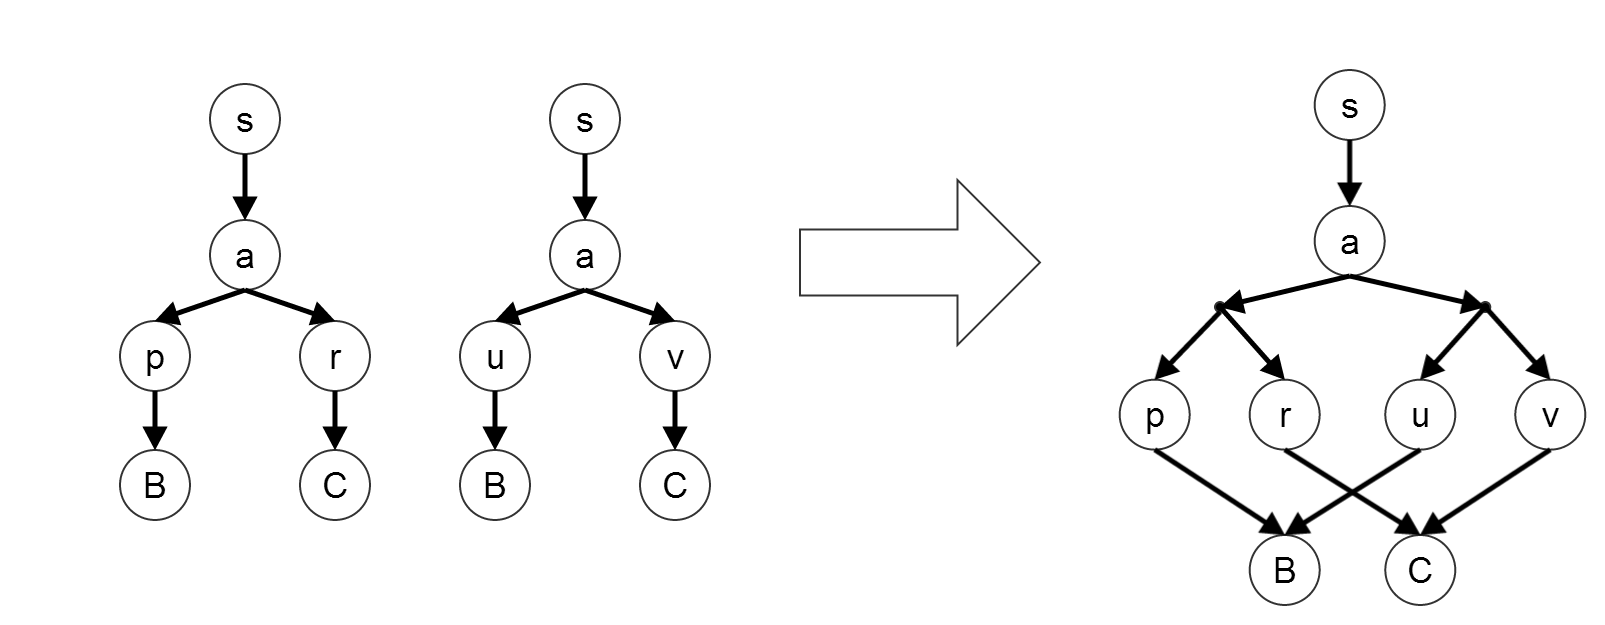
\includegraphics[width=150mm]{Pictures/sppf.png}
\caption{Пример получения SPPF из нескольких деревьев.}
\label{sppf_idea}
\end{figure}

Однако в абстрактном синтаксическом анализе возможна ещё одна ситуация. Предположим, что в грамматике только один стартовый нетерминал (если их несколько, то можно добавим новое стартовое правило). Если деревья соответствуют разным путям во входном графе, то из их корневых вершин выводятся разные цепочки. Однако некоторая часть дерева, соответствующая одному или нескольким путям от корня дерева, повторяются у всех деревьев. Поэтому такие вершины тоже предлагается сливать в одну, несмотря на то что формально они могут выводить разные цепочки. 

Поясним на примере такой грамматики.

[<Start>] 

s : a 

a : b | d 

b : A B

d : A D 

Предположим, что на входе у нас граф, изображённый на рисунке ~\ref{sppf_input}.

\begin{figure}[h]
\centering
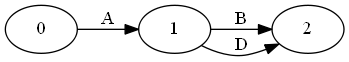
\includegraphics[width=80mm]{Pictures/SPPF_input.png}
\caption{Пример входного графа.}
\label{sppf_input}
\end{figure}

Построятся два дерева, у которых пути от вершины s до вершины a будут совпадать (см. рис. ~\ref{sppf2}). Несмотря на то что в одном дереве эти вершины выводят строку “A B”, а в другом “A D”, вершины этого пути будут также склеены в одну. 

\begin{figure}[h]
\centering
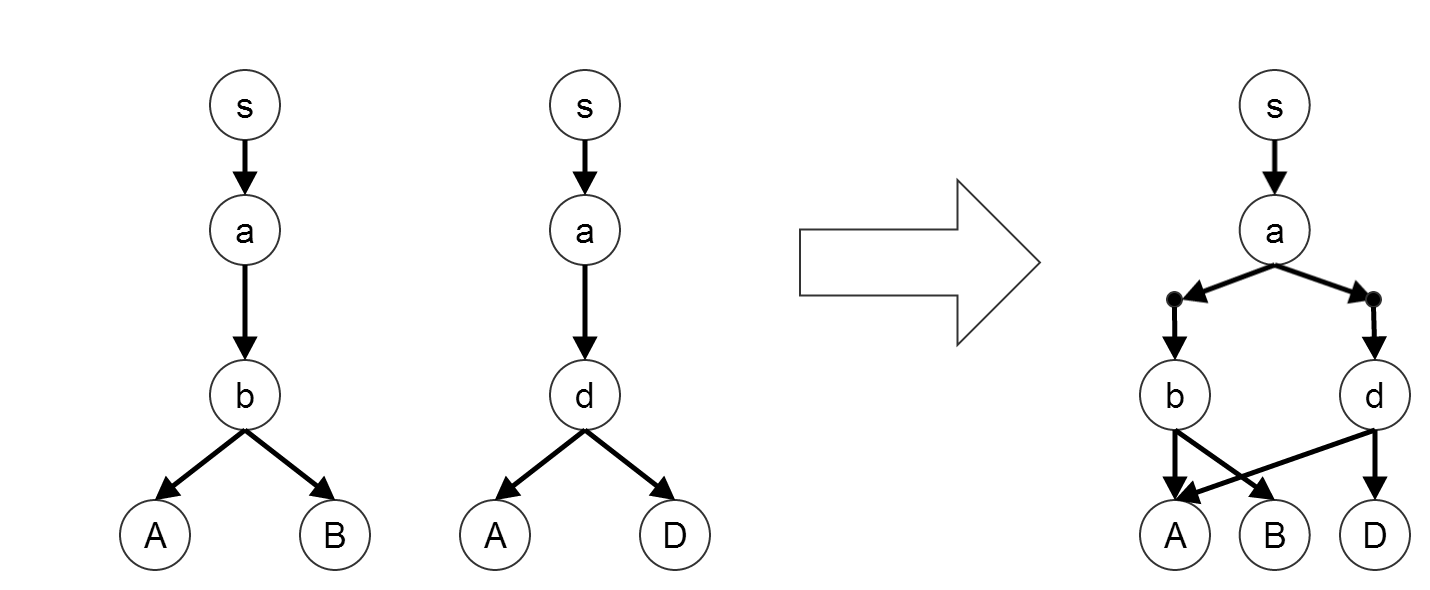
\includegraphics[width=150mm]{Pictures/sppf2.png}
\caption{Пример слияния деревьев в SPPF в абстрактном случае.}
\label{sppf2}
\end{figure}

На рисунке ~\ref{sppf_yc} показано, как будет выглядеть SPPF для предыдущего примера в реализации YaccConstructor. Заметим, что в реализации YaccConstructor у SPPF помимо привычных узлов, соответствующих терминалам и нетерминалам (далее будем называть их “вершинами-символами”), есть ещё промежуточные узлы, которые содержат в себе номера продукции (далее будем называть такие вершины “вершинами-продукциями”). 

\begin{figure}[h]
    \centering
    \begin{subfigure}{0.25\textwidth}
        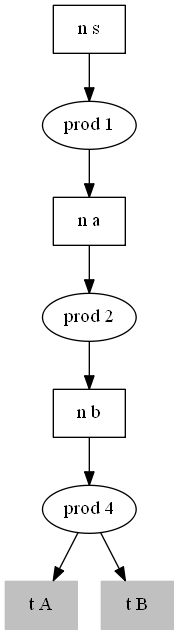
\includegraphics[height=100mm]{Pictures/SPPF_YC_ex1.png}
        \caption*{Первое дерево}
    \end{subfigure}
    \qquad
    \begin{subfigure}{0.25\textwidth}
        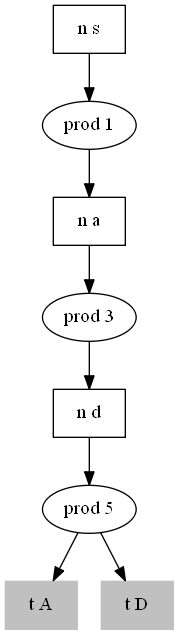
\includegraphics[height=100mm]{Pictures/SPPF_YC_ex2.png}
        \caption*{Второе дерево}
    \end{subfigure}
    \qquad
    \begin{subfigure}{0.25\textwidth}
        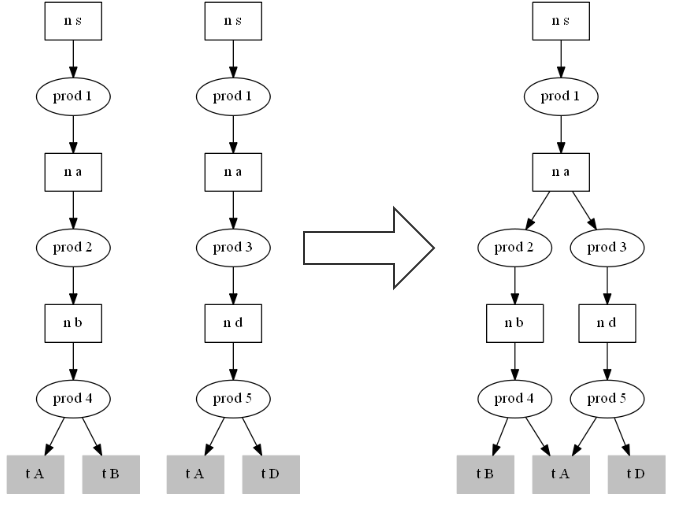
\includegraphics[height=100mm]{Pictures/SPPF_YC.png}
        \caption*{Результат слияния}
    \end{subfigure}
    \qquad
    \caption{Слияние деревьев в SPPF в YaccConstructor.}
    \label{sppf_yc}
\end{figure}

Выпишем некоторые свойства SPPF, реализованного в YaccConstructor. 
\begin{itemize}
\item Корни всех деревьев соответствуют одному и тому же нетерминалу. Поэтому при склеивании деревьев будет одна вершина, в которую не входит ни одна дуга. Далее будем называть такую вершину корнем SPPF, или просто корнем. 
\item Все токены располагались на листьях деревьев. В SPPF токены располагаются, т.е. на вершинах, из которых не выходит ни одной дуги.
\item При обходе графа от корня обнаружить вершину-символ, которую разделяют несколько поддеревьев, достаточно просто: из таких вершин выходит более одной дуги к вершинам-продукциям. 
\end{itemize}

Невозможна ситуация, когда SPPF содержит “лишние деревья”, то есть деревья, для которых нет пути во входном графе. Это свойство вытекает из построения SPPF. 

Пусть $m$ различных поддеревьев склеиваются к вершине, соответствующей одинаковому нетерминалу $n$. Тогда по построению SPPF будет создано $m$ вершин-продукций, к каждой из которых будет вести дуги из $n$. Если в дальнейшем пути от этих вершин-продукций не пересекаются, то никаких новых деревьев появиться не может. 

Таким образом, “лишнее дерево” может случиться только в случае, если какие-то деревья имеют общее поддерево. Рассмотрим это поддерево поподробнее. Если оно не содержит в себе неоднозначностей (т.е. ситуации, когда из вершины-символа выходит более, чем одна дуга, к вершинам-продукциям), то мы получим ровно столько же деревьев, сколько и разделяет это поддерево. Поэтому “лишнего” дерева в таком случае получиться не может. 

Предположим, что это поддерево содержит в себе неоднозначности и при этом была порождено лишнее дерево. Рассмотрим входной граф (рис. ~\ref{sppf_proof_input}). 

Грамматика выглядит так:

[<Start>]

s: a | b

a : A c

b: A D c

c: B | E F

\begin{figure}[h]
\centering
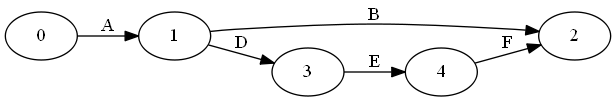
\includegraphics[width=100mm]{Pictures/SPPF_proof_input.png}
\caption{Входной граф.}
\label{sppf_proof_input}
\end{figure}

\begin{figure}[h]
    \centering
    \begin{subfigure}{0.25\textwidth}
        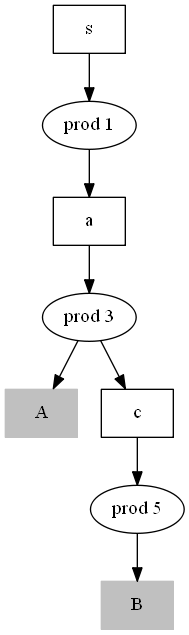
\includegraphics[height=100mm]{Pictures/SPPF_proof_fst}
        \caption*{Первое дерево}
    \end{subfigure}
    \qquad
    \begin{subfigure}{0.25\textwidth}
        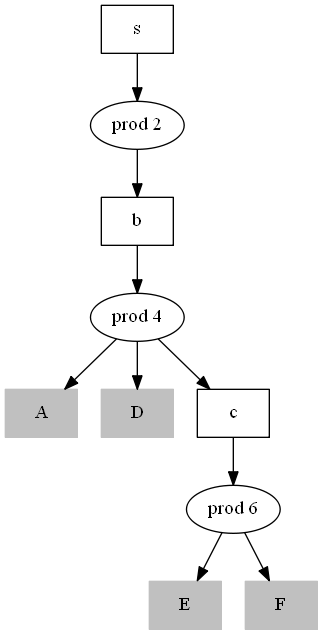
\includegraphics[height=100mm]{Pictures/SPPF_proof_snd}
        \caption*{Второе дерево}
    \end{subfigure}
    \qquad
    \begin{subfigure}{0.25\textwidth}
        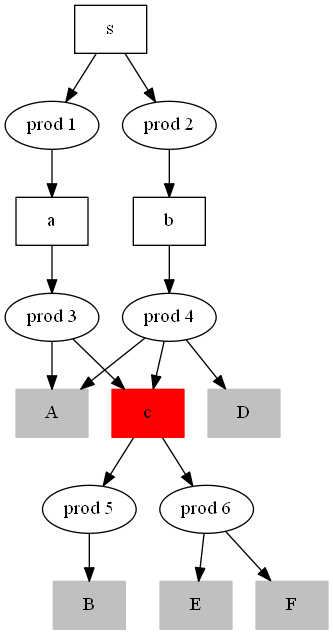
\includegraphics[height=100mm]{Pictures/SPPF_proof_incorrect.png}
        \caption*{Слияние деревьев}
    \end{subfigure}
\caption{Неправильное слияние деревьев.}
\label{sppf_proof_incorrect}
\end{figure}

В возможном SPPF (рисунок ~\ref{sppf_proof_incorrect}) два дерева (одно порождает строку “A B”, а другое - строку “A D E F”) имеют общее поддерево, начинающееся с вершины c. Причём это поддерево содержит в себе два разных поддерева: одно порождает строку “B”, а другое - строку “E F”. Таким образом, мы можем получить сразу четыре дерева разбора, которые выводят такие строки:
\begin{itemize}
\item “A B”,
\item “A E F”,
\item “A D B”,
\item “A D E F”.
\end{itemize}

Причём только для первого и четвёртого случая существуют пути в графе. 

Но граф разбора, изображённый на рисунке ~\ref{sppf_proof_incorrect}, получиться не может. Потому что нарушается требование того, что вершины сливаются в одну, если они выводят одинаковую цепочку. В данном случае это требование нарушено: в одном дереве нетерминал c выводит строку “B”, а в другом - строку “E F”. Поэтому сливать вершины, соответствующие вершинам c, в одну, нельзя. Правильный вариант SPPF изображён на рисунке ~\ref{sppf_proof_correct}.

\begin{figure}[h]
\centering
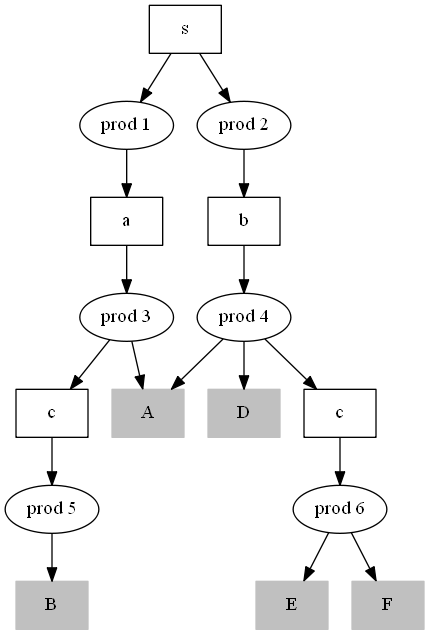
\includegraphics[height=100mm]{Pictures/SPPF_proof_correct.png}
\caption{Правильное слияние деревьев.}
\label{sppf_proof_correct}
\end{figure}

Поэтому ситуация, когда общее поддерево, содержащее неоднозначности, приводит к появлению “лишнего дерева”, невозможна. 

А значит и общая ситуация, когда SPPF содержит в себе дерево, для которого нет пути во входном графе, невозможна.
